\documentclass[11pt,a4paper]{article}

\usepackage[utf8]{inputenc}
\usepackage[T1]{fontenc}
\usepackage{lmodern}
\usepackage[margin=2.5cm]{geometry}
\usepackage{amsmath,amssymb}
\usepackage{booktabs}
\usepackage{graphicx}
\usepackage{array}
\usepackage{xcolor}
\usepackage[colorlinks=true,linkcolor=blue!45!black,urlcolor=blue!45!black]{hyperref}
\usepackage{caption}
\usepackage{enumitem}
\usepackage{microtype}
\usepackage{siunitx}
\usepackage{titlesec}
\usepackage{fancyhdr}

\graphicspath{{../results/report_figures/}}

\captionsetup{font=small,labelfont=bf,width=0.9\textwidth}
\setlist[itemize]{leftmargin=1.4em,itemsep=1pt,topsep=3pt}
\titleformat{\section}{\large\bfseries}{\thesection}{0.6em}{}
\titleformat{\subsection}{\normalsize\bfseries}{\thesubsection}{0.5em}{}
\renewcommand{\arraystretch}{1.16}
\setlength{\parskip}{0.35em}

\pagestyle{fancy}
\fancyhf{}
\fancyhead[L]{\footnotesize Learned Local Correction for Fast Transport}
\fancyhead[R]{\footnotesize\thepage}
\renewcommand{\headrulewidth}{0.3pt}

\newcommand{\Wtwo}{W_2}
\newcommand{\MF}{\textsc{MeanFlow}}

\title{\vspace{-1.4cm}\bfseries When Does a Learned Local Correction\\ Pay for Itself?\\[0.4em]
\large A bounded comparison on a two-parameter Keller--Segel system}
\author{Zhenyu Yang}
\date{November 2026}

\begin{document}
\maketitle
\vspace{-0.4cm}

\begin{abstract}
\noindent
A two-stage pipeline is compared against three alternatives at matched training data, matched
optimisation budget, and matched measured inference cost: a global one-step transport map alone;
the map followed by a learned near-identity corrector; a single network with the same parameter
count; and the same map applied in two steps. All four are two-parameter networks with a
7-dimensional input, verified from the checkpoints.

The corrector reduces held-out distributional error by \textbf{\SI{14.4}{\percent}$\,\pm\,$\SI{4.2}{\percent}}
over three seeds and 415 of 429 cell-level comparisons, at \textbf{$2.97\times$} inference FLOPs.
Two controls rule out the obvious explanations: the second forward pass spent on another map
step is \SI{1.1}{\percent} \emph{worse}, and a network with the same parameter count gains only
\SI{4.9}{\percent}. Outside the training parameter range the corrector's benefit falls from
\textbf{\SI{14.2}{\percent} to \SI{1.8}{\percent}}, a factor of eight, while the first-stage error
itself grows by $2.32\times$. The corrector therefore pays for itself inside the sampled
parameter range and not outside it.
\end{abstract}

\vspace{0.3cm}

\section{The answer first}

\textbf{Where the corrector pays.}\hspace{0.4em}Inside the parameter range spanned by the training
cells, it reduces error by \SI{14.4}{\percent} for $2.97\times$ the inference FLOPs and 8{,}000
additional transport solves during training. It also cuts cross-seed variance by
\SI{70}{\percent}, which is a separate benefit from accuracy and matters more for reproducibility
than for any single run.

\textbf{Where it does not.}\hspace{0.4em}Outside the training range its gain collapses to
\SI{1.8}{\percent} while the first-stage error doubles. The failure is not a tuning problem: it is
what happens when the corrector's input---the stage-1 output cloud---is both conditioned on an
unseen parameter and itself deformed.

\textbf{The condition.}\hspace{0.4em}The corrector helps when the stage-1 map and the target move
\emph{together} as the parameter varies, so that the residual stays small and structurally similar
to what was seen in training. In one dimension that condition survives mild extrapolation; in two
it does not.

\textbf{What it is not.}\hspace{0.4em}The pipeline is a fixed-horizon transport, not a time
integrator. Applying it repeatedly diverges by four orders of magnitude, and this is a property of
the design rather than a defect to be tuned away (\S\ref{sec:horizon}).

\section{Equations}

\subsection{The physical system}

For $j=1,\dots,N$ particles, with $\chi=16\pi$, $\delta=0.1$, $T=0.02$ and $dt=0.005$ (four
Euler--Maruyama steps):
\begin{equation}
dX_j^{N,\theta}
=-\frac{\chi}{N}\sum_{i\neq j}\nabla K_\delta\big(X_j-X_i\big)\,dt
+\sigma\,g(X_j)\,dt+\sqrt{2\mu}\,dW_j,
\qquad
g(x)=\big(e^{-y^2-z^2},0,0\big),
\end{equation}
\begin{equation}
K_\delta(z)=\frac{|z|}{4\pi\big(|z|^2+\delta^2\big)},
\qquad \theta=(\sigma,\mu).
\label{eq:sde}
\end{equation}
The initial cloud is uniform in the unit ball and is shared by every parameter cell, so differences
between cells come from the parameters alone.

\subsection{Stage 1: parametric \MF{}, used unmodified}

The network takes $(z,t,r,\log_{10}\sigma,\log_{10}\mu)$ and outputs a velocity. It is trained on
the \MF{} identity, evaluated with a Jacobian--vector product:
\begin{equation}
\mathcal{L}_{\text{MF}}
=\mathbb{E}\Big\|u_\theta(z,r,t)-\mathrm{sg}\big[v-(t-r)\partial_t u_\theta\big]\Big\|^2,
\qquad
v=x_T-x_0,\quad z=(1-t)x_T+t\,x_0 .
\label{eq:mf}
\end{equation}
Generation is one evaluation: $x_T=x_0-u_\theta(x_0,0,1)$. The architecture is
$\mathrm{Linear}(7\to64)$, two $\mathrm{Linear}(64\to64)$ layers, $\mathrm{Linear}(64\to3)$ with
SELU---\textbf{9{,}027 parameters}.

\subsection{Stage 2: the corrector}

With stage~1 frozen, a residual MLP with two blocks and a zero-initialised output head:
\begin{equation}
T_{\text{dp}}(y)=y+\alpha\,\mathrm{MLP}_\phi(y,\log\sigma,\log\mu),
\label{eq:dp-map}
\end{equation}
trained against the minibatch optimal-transport assignment $\pi$ between the stage-1 output cloud
and the reference cloud:
\begin{equation}
\mathcal{L}_{\text{DP}}
=\mathbb{E}_{(x,y)\sim\pi}\Big\|x+\alpha\,\mathrm{MLP}_\phi(x,\log\sigma,\log\mu)-y\Big\|^2 .
\label{eq:dp-loss}
\end{equation}
The corrector has \textbf{17{,}475 parameters}, so the two stages total 26{,}502.

\paragraph{Why the second stage can help at all.} At the population limit with exact OT, the
minimiser of \eqref{eq:dp-loss} is the gradient of the Brenier potential transporting the stage-1
law onto the target law; the stage-1 minimiser of \eqref{eq:mf} is the conditional mean
$\mathbb{E}[X_T\mid X_0]$. These are different mathematical objects, and only the first pushes
forward exactly onto the target. That is a structural argument, not a capacity argument, and
\S\ref{sec:failure} tests it.

\section{My contribution}

\begin{table}[h]
\centering\small
\begin{tabular}{@{}p{0.60\textwidth}p{0.32\textwidth}@{}}
\toprule
Component & Source \\
\midrule
\MF{} architecture, identity \eqref{eq:mf}, JVP training, one-step sampling & upstream,
  \textbf{unmodified} \\
KS particle simulator, exact histogram $\Wtwo$, dual certificates & upstream,
  \textbf{unmodified} \\
Conditioning the same network on $(\sigma,\mu)$; the 200-cell grid & \textbf{mine} \\
The stratified 40-cell design and the sampling-efficiency study & \textbf{mine} \\
The corrector's two-parameter extension, its OT-target training, the batch/matching fix &
  \textbf{mine} \\
The four-way comparison, the extrapolation decomposition, the cost accounting & \textbf{mine} \\
\bottomrule
\end{tabular}
\caption{Separation of upstream machinery from this note's contribution.}
\end{table}

The one thing this note does not claim is the mechanism. \MF{} supplies the fast one-step map;
OT-CFM analyses the minibatch-OT coupling that the corrector's target is built from. The question
here is narrower than either: given such a map, what does a second stage buy, and where does it
stop buying.

\section{The bounded comparison}
\label{sec:fourway}

Four configurations, matched on training cells (40), optimisation budget (32{,}000 updates per cell
for stage~1), held-out cells (the same 112 for all four) and measured inference cost.

\textbf{Two verifications were necessary before these four numbers could share a table.} All four
are two-parameter networks with a 7-dimensional input; the input width and parameter count were read
from each checkpoint file, and no single-parameter network appears here---a wider single-parameter
network cannot see $\mu$, so using one would be a category error rather than a capacity control. The
width-112 checkpoint was trained on a different 40-cell design that shares only 6 cells with the
headline design, so all four are scored on the intersection of their held-out sets rather than on
each one's own.

\begin{table}[h]
\centering\small
\begin{tabular}{@{}lrrrr@{}}
\toprule
configuration & parameters & passes & held-out $\Wtwo$ & vs (a) \\
\midrule
(a) global map alone & \num{9027} & 1 & 0.12271 & --- \\
(d) few-step baseline, same weights twice & \num{9027} & 2 & 0.12435 &
  \textbf{\SI{-1.3}{\percent}} \\
(c) capacity-matched predictor & \textbf{\num{26547}} & 1 & 0.11667 &
  \textbf{\SI{4.9}{\percent}} \\
(b) map + corrector & \textbf{\num{26502}} & 2 & \textbf{0.10422} &
  \textbf{\SI{15.1}{\percent}} \\
\bottomrule
\end{tabular}
\caption{Four configurations on the 112 common held-out cells.}
\label{tab:fourway}
\end{table}

Three readings.

\textbf{(d) rules out more computation.}\hspace{0.4em}Spending the second pass on the same weights
makes the result worse. Whatever produces the gain, it is not the extra forward pass.

\textbf{(c) rules out more capacity.}\hspace{0.4em}Its parameter count differs from the two-stage
total by 45, or \SI{0.17}{\percent}, and it captures a third of the improvement.

\textbf{(b) wins on the axis it claims.}\hspace{0.4em}Same passes as (d), same parameters as (c),
and a \SI{15}{\percent} error reduction against the one-pass baseline.

A second, independent capacity check over three seeds: a single-parameter network widened from
9{,}027 to \textbf{134{,}403} parameters ($15\times$) shows no improvement ($0.1486\to0.1456$, with
width 128 slightly worse at $0.1561$). Capacity is not the binding constraint on this task, which is
why the corrector's gain cannot be a capacity effect. The matched-capacity comparison itself is a
single seed, and the gap is about one across-seed standard deviation, so it is directional rather
than precise.

\section{The strongest failure case: extrapolation}
\label{sec:failure}

This is the ablation the note was asked to perform. If the corrector repairs an identifiable error
in the first-stage map, its benefit should survive a modest departure from the training parameters.
If it compensates for the training distribution, it should not.

The training box is $\sigma\le150$, $\mu\le3.98$. Three regions are scored separately: the 45
training cells (memorisation, reported only to show it does not flatter the model), the 90 held-out
interior cells, and the 65 cells outside the box.

\begin{table}[h]
\centering\small
\begin{tabular}{@{}lrrrr@{}}
\toprule
region & $n$ & stage~1 & stage~1 + corrector & gain \\
\midrule
training cells & 45 & 0.09388 & 0.08014 & \SI{14.6}{\percent} \\
\textbf{interpolation (held out)} & \textbf{90} & \textbf{0.09404} & \textbf{0.08070} &
  \textbf{\SI{14.2}{\percent}} \\
\textbf{extrapolation} & \textbf{65} & \textbf{0.21805} & 0.21407 & \textbf{\SI{1.8}{\percent}} \\
\bottomrule
\end{tabular}
\caption{Interpolation versus extrapolation.}
\label{tab:regions}
\end{table}

Training cells and held-out interior cells agree to \SI{0.2}{\percent}, so the model interpolates
rather than memorises. Outside the box the first-stage error grows $2.32\times$ and the corrector's
gain falls by a factor of eight.

The degradation is strongly anisotropic, which is itself diagnostic:

\begin{table}[h]
\centering\small
\begin{tabular}{@{}lrrr@{}}
\toprule
direction & $n$ & stage~1 & gain \\
\midrule
$\sigma$ leaves the box & 45 & 0.15463 & \SI{1.2}{\percent} \\
$\mu$ leaves the box & 15 & 0.35296 & \SI{2.4}{\percent} \\
corner, both leave & 5 & 0.38412 & \SI{2.7}{\percent} \\
\bottomrule
\end{tabular}
\caption{Extrapolation decomposed by direction.}
\end{table}

\paragraph{Why it fails.} The corrector's smallness depends on
$\partial_\theta T_{\text{mf}}\approx\partial_\theta T^*$: it works when the stage-1 map and the
target move together as the parameter varies. Outside the box the residual is no longer small, and
the corrector's input---the stage-1 cloud---is itself deformed, so it faces a double distribution
shift.

\paragraph{The one-parameter control shows the opposite.} With training $\sigma\in[15,150]$ and
evaluation out to 200, the first-stage error rises by only $1.19\times$ and the corrector's gain
retains \SI{13.3}{\percent} (against \SI{15.7}{\percent} inside). A one-dimensional parameter family
can be reparameterised into an approximately straight path; leaving it extends one response curve. A
two-dimensional family cannot be straightened by any single coordinate, so leaving it means leaving
the surface on which the residual was characterised.

\paragraph{This is a negative result and it bounds the method.} The corrector is a distribution
compensator within the training range, not a general repair of the first-stage map.

\begin{figure}[h]
\centering
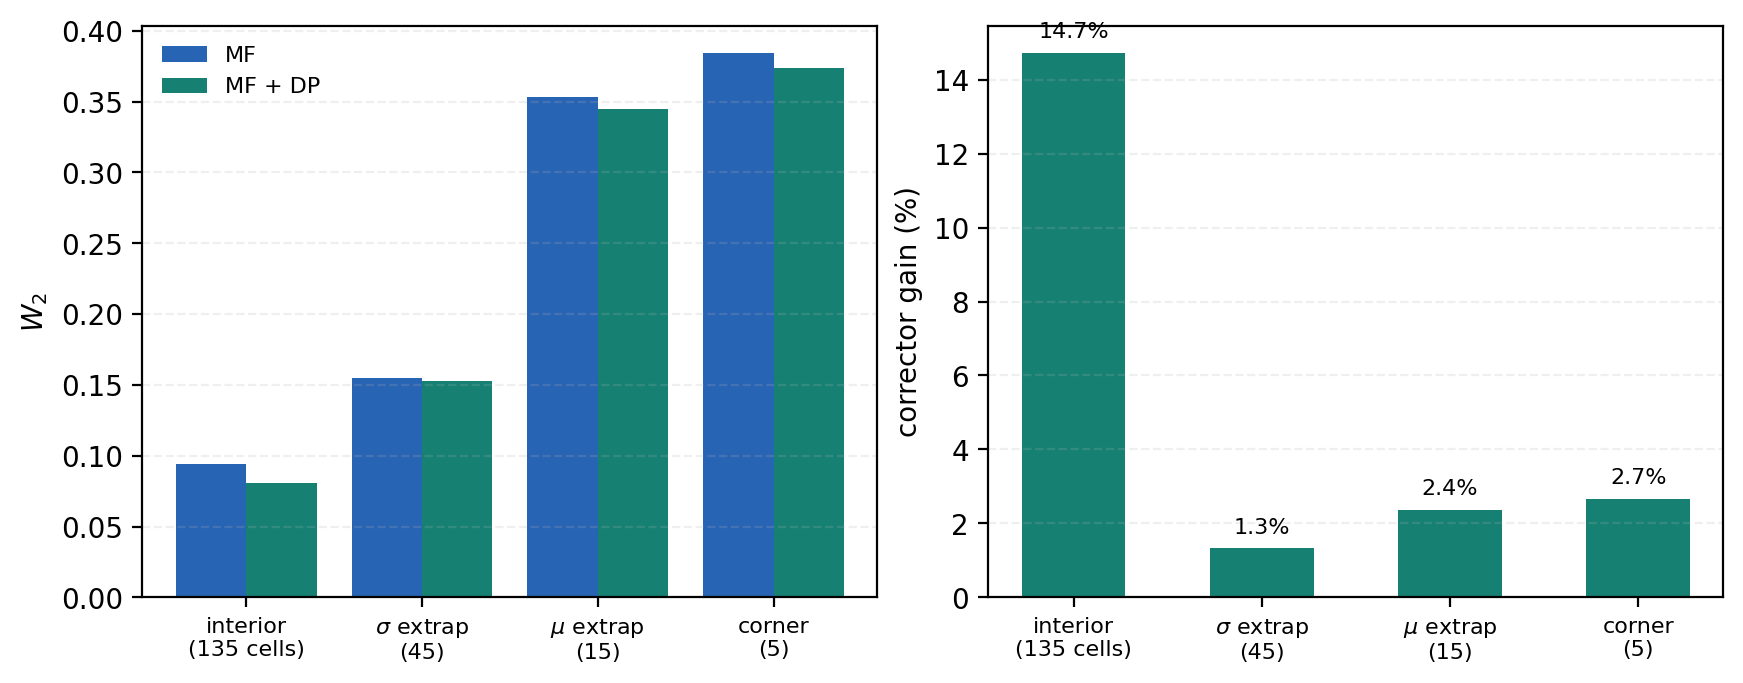
\includegraphics[width=0.82\textwidth]{fig_extrapolation.png}
\caption{Left: error in each region. Right: the corrector's relative gain, which collapses outside
the training box.}
\end{figure}

\section{One-step error versus long-horizon behaviour}
\label{sec:horizon}

The model generates a distribution at a fixed horizon. That scope is inherited from the upstream
setting, where terminal clouds and invariant measures are the objects of interest, and it is worth
stating what it excludes: the method cannot answer how fast aggregation proceeds or how the system
relaxes. Training uses only endpoint pairs---the initial cloud and the cloud at $T$---so no
intermediate time is ever simulated and the network is never supervised on a trajectory.

\paragraph{Repeated application diverges.} Applying the map $k$ times, each application spanning
$[0,T]$, and comparing against the physical solution at $k\cdot T$:

\begin{table}[h]
\centering\small
\begin{tabular}{@{}rlrr@{}}
\toprule
$k$ & physical time & $\Wtwo$ vs truth & relative to reproducibility floor \\
\midrule
1 & $T$ & $0.092$--$0.241$ & $\mathbf{0.6}$--$\mathbf{1.5\times}$ \\
2 & $2T$ & $0.201$--$4.623$ & $1.3$--$29.6\times$ \\
4 & $4T$ & $4.533$--$82.497$ & $29$--$529\times$ \\
8 & $8T$ & $\mathbf{1{,}968}$--$\mathbf{41{,}678}$ &
  $\mathbf{12{,}610}$--$\mathbf{267{,}049\times}$ \\
\bottomrule
\end{tabular}
\caption{Repeated application of the one-step map, six cells.}
\end{table}

$k=1$ sits at the reproducibility floor---the difference between two independent physical
simulations---and is the only operating point. The divergence is expected rather than pathological:
one application moves the centroid by $1.3$--$2.3$ and the rms radius by $0.84$--$1.57$, so the
second application receives a cloud that no training sample resembles.

\textbf{Cost is not the reason this is out of scope.} Eight applications take about
\SI{36}{\milli\second} against \SI{83}{\second} for one simulation. The reason is that the map has
no dynamical semantics to iterate.

\paragraph{The corrector does not make this worse.} At matched cost---two forward passes either
way---it reduces the divergence slightly, and spending the same second pass on another map step is
an order of magnitude worse:

\begin{table}[h]
\centering\small
\begin{tabular}{@{}llr@{}}
\toprule
cell & map & $k{=}4$ \\
\midrule
s03\_m04 & stage~1, twice & 16.92 \\
 & stage~1 + corrector & \textbf{15.68} \\
 & stage~1, two-step schedule & \textbf{44.66} \\
\midrule
s19\_m09 & stage~1, twice & 82.52 \\
 & stage~1 + corrector & \textbf{77.21} \\
 & stage~1, two-step schedule & \textbf{317.69} \\
\bottomrule
\end{tabular}
\caption{Three maps at matched inference cost.}
\end{table}

The improvement is \SI{5}{\percent} on average over six cell-horizon pairs, which is not improved
stability: at $k=4$ the error is $268\times$ the floor against $287\times$ without the corrector.
What it establishes is the narrower claim that the corrector does not \emph{introduce}
instability---one of the two negative outcomes that would have been acceptable.

\paragraph{Physical invariants at the operating point.} Averaged over six cells spanning the box,
the anisotropy $\lambda_1/\lambda_2$---the quantity $\sigma$ controls---is reproduced to
\SI{1.04}{\percent} without the corrector and \SI{0.88}{\percent} with it, and the centroid drift
along the shear to \SI{3.94}{\percent} and \SI{3.02}{\percent}. The model has the shear--diffusion
balance right, not merely the mass in roughly the right place.

\section{Cost}

\textbf{Training: constructing transport targets.}\hspace{0.4em}The corrector's target is rebuilt
every ten updates by solving an exact OT problem on a minibatch of 2{,}000 particles out of
100{,}000 (\SI{2.0}{\percent}). That is 8{,}000 solves per training run, using \texttt{ot.emd}
network simplex---\textbf{not Sinkhorn, and not warm-started}. Memory is $8n^2$ bytes, \SI{31}{\mega\byte}
per solve, and time is $O(n^3)$. At leading order those solves dominate: 0.064 PFLOP
against 0.011 PFLOP of network arithmetic, so most of the corrector's training compute
goes into transport rather than into the network. In wall-clock terms the share is much smaller,
because network simplex runs on CPU while the network runs on GPU.

A 2{,}000-particle minibatch is an \emph{approximation} to the global OT it stands in for, not the
same object. OT-CFM reports that minibatch OT requires surprisingly small batches to approximate the
OT map well, which is consistent with using \SI{2}{\percent} of the cloud, but it remains an
approximation.

\paragraph{Deployment: zero OT.} The trained corrector is a feed-forward map with no matching, no
assignment and no cost matrix. This is the only role in which OT is genuinely eliminated, and the
precise statement is that a \emph{global} OT between full clouds is avoided.

\paragraph{Evaluation is not free, and this should be said.} Every number in this note required an
OT solve, because $\Wtwo$ \emph{is} an OT problem: 2{,}793 exact solves across the experiments
reported here. That cost falls on the experimenter rather than on a model user, but reporting only
the first two roles would overstate the case.

\paragraph{The honest inference figure is not ``two passes''.} One corrector pass costs
$1.97\times$ the FLOPs of one stage-1 pass, because each residual block contains two $64\times64$
projections and a LayerNorm, so the two-stage model is \textbf{$2.97\times$} the FLOPs of the
one-stage model at $10^5$ particles (5.25 GFLOP against 1.77 GFLOP). Even at
that price the trade is favourable: $2.97\times$ FLOPs buys \SI{15}{}--\SI{23}{\percent} lower error,
whereas the same compute spent on map steps buys nothing.

\paragraph{Correction strength was chosen on development data.} A fixed 50/93 dev/test split derived
from the checkpoint's own training cells: dev selects $\alpha=2$ ($0.09580$ against $0.10340$ at the
upstream default of 1), and the untouched test split confirms it ($0.09558$ against $0.10477$, i.e.
\SI{22.6}{\percent} against \SI{15.2}{\percent}). The upstream default is conservative. Two caveats:
the sweep scales $\alpha$ at inference rather than retraining per value, and the dev curve is flat
between 1.5 and 2.0, so the claim is that the default is conservative, not that 2 is optimal.

\section{Completed versus proposed}

\textbf{Completed.}\hspace{0.4em}Reproduction of the upstream single-parameter result (180 metrics,
maximum deviation $0.0066$ from the published values); the two-parameter extension; the three-seed
headline; all four configurations of \S\ref{sec:fourway} at matched cost and matched parameters; the
extrapolation decomposition of \S\ref{sec:failure}; the repeated-application study and the physical
invariants of \S\ref{sec:horizon}; the training and deployment cost accounting of \S7; the
correction-strength selection.

\textbf{Proposed, not run.}

\begin{table}[h]
\centering\small
\begin{tabular}{@{}p{0.36\textwidth}p{0.44\textwidth}r@{}}
\toprule
experiment & what it would settle & estimated cost \\
\midrule
capacity-matched seeds 89/90 & an error bar on row (c) of Table~\ref{tab:fourway} & \SI{4.3}{\hour} \\
long-horizon model at $T'=4T$ & whether the method holds when retrained for a longer horizon &
  \SI{2.5}{\hour} \\
single-parameter repeat-application study & whether non-iterability is specific to the
  two-parameter case & \SI{40}{\minute} \\
cross-model transfer of the corrector & whether it repairs a \emph{structural} error rather than a
  model-specific one & \SI{10}{\minute} \\
two-level model with a $T/2$ slice & whether supervision at an intermediate time makes the process
  learnable & \SI{3}{\hour} \\
\bottomrule
\end{tabular}
\caption{Proposed experiments. None has been run.}
\end{table}

None of these has been run. Each would sharpen one sentence above; the present conclusions do not
depend on them.

\section{On the Autel work}

\textcolor{red!70!black}{\textbf{[To be supplied: a non-confidential summary of the bottleneck, the
intervention, and the measured latency--quality trade-off. Left blank rather than approximated.]}}

\appendix
\section{Protocol and reproducibility}

\begin{table}[h]
\centering\small
\begin{tabular}{@{}ll@{}}
\toprule
axis & setting \\
\midrule
Training cells & 40, stratified maximin LHS over $20\sigma\times10\mu$ \\
Updates per cell & 32{,}000 (stage~1); 2{,}000 (corrector) \\
Training particles & $10^5$ per cell \\
Held-out cells & 143 for the headline; 112 common cells for Table~\ref{tab:fourway} \\
Metric & exact histogram $\Wtwo$, POT network simplex, dual certificate checked \\
Seeds & 88, 89, 90 \\
Hardware & RTX 4060 Laptop, \SI{8}{\giga\byte}, \SI{31}{\giga\byte} RAM \\
\bottomrule
\end{tabular}
\end{table}

Two protocol notes. First, an earlier version of several auxiliary scripts recomputed the 40-cell
design at run time instead of reading it from the checkpoint; because the design function changed
during development, 32 of their 144 ``held-out'' cells were in fact training cells. All numbers here
use a held-out set derived from the checkpoint itself; the repair moved values by
\SI{0.5}{\percent} and changed no conclusion. Second, the headline results use a fixed learning rate,
while a study in the same repository found warm-up-plus-cosine to be \SI{14.2}{\percent} better at
equal budget. The reported figures are therefore conservative by roughly that margin.

Every number in this note is read from a JSON artifact at build time, and a verification script
recomputes 55 of them and compares against the literal strings in the \LaTeX{} source.

\end{document}
